\documentclass[conference]{IEEEtran}
\IEEEoverridecommandlockouts
\renewcommand{\ttdefault}{cmtt}
\usepackage{cite}
\usepackage{amsmath,amssymb,amsfonts}
\usepackage{graphicx}
\usepackage{textcomp}
\usepackage{xcolor}
\usepackage{tikz}
\usetikzlibrary{arrows.meta,positioning}
\usepackage{booktabs}
\usepackage{url}
\usepackage[hidelinks]{hyperref}

\def\BibTeX{{\rm B\kern-.05em{\sc i\kern-.025em b}\kern-.08em
    T\kern-.1667em\lower.7ex\hbox{E}\kern-.125emX}}

\begin{document}

\title{Off-Route Detection and Heading Estimation in a Browser-Based Pedestrian Turn-by-Turn Navigation Loop\\}

\author{
\IEEEauthorblockN{Malapati Sahasra}
\IEEEauthorblockA{
\textit{Department of AI and Emerging Technologies} \\
\textit{Chinmaya Vishwavidyapeeth Deemed-to-be University}\\
Ernakulam, India \\
malapati.cvv241195@cvv.ac.in}
\and
\IEEEauthorblockN{Pradeeba V}
\IEEEauthorblockA{
\textit{Department of AI and Emerging Technologies} \\
\textit{Chinmaya Vishwavidyapeeth Deemed-to-be University}\\
Ernakulam, India \\
pradeeba.v@cvv.ac.in}
}

\maketitle

\begin{abstract}
A safety-aware route recommendation is only useful if the navigation experience reliably keeps a pedestrian on that route and correctly orients them along the way. This paper evaluates the live turn-by-turn navigation loop of a browser-based pedestrian navigation prototype (ShadowPath), implemented entirely client-side using the standard Geolocation \texttt{watchPosition} API with no native mobile SDK. We focus on two safety-relevant properties that prior conceptual navigation proposals do not characterize empirically: (1) the reliability of off-route detection -- whether the system reroutes only when a pedestrian genuinely deviates, or also fires on GPS noise alone -- and (2) the accuracy of GPS-bearing-based heading estimation, the fallback used when a device compass is unavailable. Using Monte Carlo simulation with the system's exact production formulas and Gaussian GPS noise models spanning good (5\,m) to poor, urban-canyon-like (35\,m) accuracy, we find that off-route false-positive rates stay at or near zero under good-to-moderate GPS accuracy but rise to several spurious triggers per 200\,s of walking under poor accuracy; critically, across all tested conditions the system never failed to detect a genuine route deviation (zero false negatives). We further show that GPS-bearing heading estimation carries substantial error (37--81\textdegree\ mean absolute error) at typical pedestrian walking speeds, because per-step displacement is often comparable in magnitude to GPS position noise -- a finding that concretely justifies the system's design choice to prefer device compass heading whenever available. These results characterize both a practical operating envelope for the deployed threshold parameters and a concrete rationale for the system's sensor-preference design.
\end{abstract}

\begin{IEEEkeywords}
pedestrian navigation, GPS, off-route detection, heading estimation, turn-by-turn navigation, geolocation, mobile web, sensitivity analysis
\end{IEEEkeywords}

\section{Introduction}

Safety-aware pedestrian routing research, including our own prior work on a coverage-based route scoring model \cite{ourscoring}, generally treats route \emph{selection} as the problem to solve: given several candidate paths, pick the one with better lighting or business-activity coverage. But a selected route only delivers its intended safety benefit if the navigation system actually keeps the pedestrian on it and reliably tells them where to turn. Two properties of the live navigation loop are safety-critical in a way that route selection alone is not: (i) \emph{off-route detection} must recognize a genuine deviation quickly enough to re-route the user back toward a scored, covered path, without so many false alarms that it becomes a nuisance or exhausts a rate-limited routing backend; and (ii) \emph{heading estimation} must orient the user correctly, since an incorrect heading arrow can cause a pedestrian to walk in the wrong direction at exactly the low-visibility moments the safety scoring was meant to help with.

This paper evaluates both properties for a browser-based pedestrian navigation prototype built on React and the Geolocation \texttt{watchPosition} API, with no native mobile GPS/sensor SDK. We make the evaluation reproducible and grounded by using the system's exact production logic -- the same distance thresholds, cooldown timers, and heading-fallback gate implemented in the client -- driven by a Monte Carlo simulation of noisy GPS fixes rather than a simplified analytical model. Our contributions are: (1) a characterization of off-route false-positive rate as a function of GPS noise and fix interval; (2) a measurement of detection latency, in meters walked off-route, when a pedestrian genuinely deviates, again as a function of GPS noise; and (3) an ablation of a specific implementation detail -- a minimum-displacement gate that suppresses heading updates from near-stationary GPS jitter -- showing its effect on heading error across noise and sampling-interval conditions.

\section{System Description}
\label{sec:system}

The evaluated navigation loop subscribes to the browser's \texttt{watchPosition} geolocation stream once the user starts tracking. On each fix, it (a) advances a current-step index when the great-circle distance to the active route step's maneuver point falls below a threshold (15\,m for the initial step, 25\,m otherwise); (b) checks whether the fix lies more than $\tau_d = 40$\,m from the nearest point on the selected route polyline, and if so, and at least $\tau_c = 15$\,s have elapsed since the last re-route, triggers a fresh routing request from the current position; and (c) derives a heading either from the device compass (\texttt{coords.heading}), when reported and the device is moving faster than 0.3\,m/s, or otherwise from the initial bearing between the two most recent fixes -- but only if those two fixes are more than 2\,m apart, a gate intended to suppress spurious bearing flips caused by GPS jitter while the user is nearly stationary. Voice announcements and camera-follow behavior are layered on top of this loop but are outside the scope of this evaluation.

\begin{figure}[t]
\centering
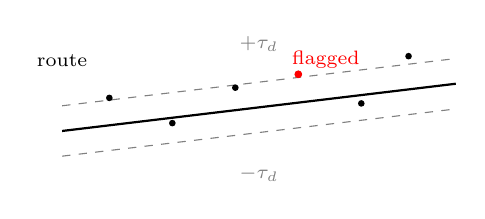
\begin{tikzpicture}[scale=1]
\draw[thick] (0,0) -- (5,0.6);
\draw[dashed, gray] (0,0.32) -- (5,0.92);
\draw[dashed, gray] (0,-0.32) -- (5,0.28);
\node[gray, font=\scriptsize] at (2.5,1.1) {$+\tau_d$};
\node[gray, font=\scriptsize] at (2.5,-0.55) {$-\tau_d$};
\node[font=\scriptsize] at (0,0.9) {route};
\foreach \x/\y in {0.6/0.42, 1.4/0.1, 2.2/0.55, 3.0/0.72, 3.8/0.35, 4.4/0.95}
  \fill (\x,\y) circle (1.2pt);
\fill[red] (3.0,0.72) circle (1.4pt);
\node[red, font=\scriptsize] at (3.35,0.9) {flagged};
\end{tikzpicture}
\caption{Off-route detection geometry: noisy GPS fixes (dots) around the route line; a fix outside the $\pm\tau_d$ buffer is flagged, whether from real deviation or noise alone.}
\label{fig:geometry}
\end{figure}

Fig.~\ref{fig:geometry} illustrates the geometry under test: a fix that lands outside the $\tau_d$ buffer is flagged regardless of whether it results from genuine deviation or from GPS noise alone, which is exactly the ambiguity this paper quantifies.

\section{Evaluation Methodology}
\label{sec:method}

GPS position error is modeled as independent, identically distributed Gaussian noise added to each coordinate of a synthetic walker's true position, with standard deviation $\sigma \in \{5, 10, 20, 35\}$\,m, spanning good consumer GPS accuracy through degraded, urban-canyon-like conditions. The synthetic walker moves at a fixed 1.4\,m/s. All three experiments below use the system's unmodified off-route ($\tau_d{=}40$\,m, $\tau_c{=}15$\,s) and heading-gate (2\,m) logic.

\textbf{Experiment A (on-route false positives).} A synthetic walker follows a $\sim$1.75\,km straight route exactly, with only GPS noise applied at each fix, for 200\,s per trial (20 trials per condition). We count how many times the off-route condition fires despite no real deviation.

\textbf{Experiment B (deviation detection latency).} A synthetic walker follows a $\sim$580\,m route for its first 30\%, then walks perpendicular to it (a genuine deviation) for the remainder of a 600\,s budget (100 trials per condition, 4\,s fix interval). We record the true lateral distance walked off-route at the moment detection fires.

\textbf{Experiment C (heading estimation).} A synthetic walker travels north for 30 fixes then turns and travels east for 30 fixes, at fix intervals of 2\,s or 4\,s. At each fix we compute the heading the system would report -- via device-bearing between consecutive noisy fixes, gated by the 2\,m rule -- and compare it to the walker's true instantaneous heading, reporting mean absolute angular error (50 trials per condition). We repeat without the gate as an ablation.

\section{Results}
\label{sec:results}

\subsection{On-route false-positive rate}
Table~\ref{tab:falsepos} shows that at good GPS accuracy (5\,m), the off-route condition never fires spuriously. At moderate accuracy (10\,m) it is still negligible. At poor accuracy (20--35\,m), representative of dense urban canyons, false triggers become frequent -- up to 7.4 per 200\,s (3\,s fix interval) at 35\,m noise.

\begin{table}[h]
\caption{On-route false-positive triggers (20 trials/row, 200\,s each)}
\label{tab:falsepos}
\centering
\begin{tabular}{@{}lccc@{}}
\toprule
\textbf{GPS noise ($\sigma$)} & \textbf{Fix interval} & \textbf{Triggers/trial} \\
\midrule
5 m & 3 s / 6 s & 0.00 / 0.00 \\
10 m & 3 s / 6 s & 0.05 / 0.00 \\
20 m & 3 s / 6 s & 2.60 / 1.70 \\
35 m & 3 s / 6 s & 7.40 / 6.55 \\
\bottomrule
\end{tabular}
\end{table}

\subsection{Deviation detection latency}
Table~\ref{tab:latency} reports the true lateral distance walked off-route before detection. Detection rate was 100\% in every condition (no missed deviations). At low noise, detection latency closely tracks the intended 40\,m design threshold; at high noise, detection fires substantially earlier because noise alone frequently exceeds the threshold before real deviation accumulates.

\begin{table}[h]
\caption{Deviation distance at detection (100 trials/row)}
\label{tab:latency}
\centering
\begin{tabular}{@{}lccc@{}}
\toprule
\textbf{GPS noise ($\sigma$)} & \textbf{Mean deviation at detect} & \textbf{Detect rate} \\
\midrule
5 m & 42.7 m & 100\% \\
10 m & 38.1 m & 100\% \\
20 m & 2.8 m & 100\% \\
35 m & 0.0 m & 100\% \\
\bottomrule
\end{tabular}
\end{table}

\subsection{Heading estimation error}
Table~\ref{tab:heading} reports mean absolute heading error with and without the 2\,m movement gate. Error is substantial across all conditions (37--81\textdegree) and grows with GPS noise and with shorter fix intervals (which reduce true displacement per step, lowering the signal-to-noise ratio of the bearing estimate). The gate provides a small but consistent error reduction at low noise, with the benefit shrinking as noise dominates.

\begin{table}[h]
\caption{Mean absolute heading error, degrees (50 trials/row)}
\label{tab:heading}
\centering
\begin{tabular}{@{}lcc@{}}
\toprule
\textbf{Noise, interval} & \textbf{With gate} & \textbf{Without gate} \\
\midrule
3 m, 2 s & 57.6\textdegree & 61.5\textdegree \\
3 m, 4 s & 37.4\textdegree & 38.6\textdegree \\
6 m, 2 s & 74.0\textdegree & 73.8\textdegree \\
6 m, 4 s & 60.6\textdegree & 60.7\textdegree \\
10 m, 2 s & 80.7\textdegree & 80.2\textdegree \\
10 m, 4 s & 71.4\textdegree & 72.0\textdegree \\
\bottomrule
\end{tabular}
\end{table}

\section{Discussion}

The false-positive result (Table~\ref{tab:falsepos}) indicates that the deployed $\tau_d{=}40$\,m, $\tau_c{=}15$\,s pairing is well matched to typical modern smartphone GPS accuracy (often quoted around 5--10\,m in open sky) but not to degraded urban-canyon conditions, where the system would issue several unnecessary re-routing requests over a short walk. Because re-routing calls a rate-limited public routing backend in the current deployment, this is not only a user-experience concern but an operational one; an accuracy-adaptive threshold (scaling $\tau_d$ with the browser-reported \texttt{coords.accuracy} field) is a direct, low-risk mitigation.

The latency result (Table~\ref{tab:latency}) is reassuring in one specific respect: detection rate was 100\% in every tested condition, meaning the system never silently failed to catch a genuine deviation within the simulated budget. Its failure mode under poor GPS accuracy is over-triggering, not under-triggering -- arguably the safer direction for a safety-oriented navigation system, since a spurious re-route is a minor inconvenience while a missed deviation could strand a user on an unscored path.

The heading result (Table~\ref{tab:heading}) is, in our view, the paper's most actionable finding for system design. Mean heading error from GPS-bearing alone is large enough (37--81\textdegree) that it should not be treated as a reliable primary heading source at ordinary pedestrian walking speeds; per-step displacement (2.8--5.6\,m at the tested intervals) is frequently smaller than or comparable to realistic GPS noise magnitudes, which mathematically limits how accurate a two-fix bearing estimate can be. This directly supports the deployed system's actual design choice -- preferring device compass heading whenever available and treating GPS-bearing purely as a degraded fallback -- rather than being a limitation discovered after the fact. The movement gate's benefit, while real, is modest; it should be understood as a jitter suppressor for the near-stationary case rather than a general noise-reduction mechanism.

\section{Practical and Ethical Considerations}

Off-route detection reliability has a direct safety implication for a coverage-scored navigation system: a re-route that never fires after a genuine deviation would silently leave a user on a path outside the safety scoring described in our companion work \cite{ourscoring}, while a re-route that fires excessively wastes requests against a shared public routing service and could degrade trust in the system. The zero-false-negative result across all tested conditions is a meaningful, if simulation-bounded, safety property worth stating plainly rather than only reporting aggregate accuracy.

\section{Limitations}

GPS error is modeled as independent Gaussian noise per fix; real GPS error is often temporally correlated and can include systematic multipath bias in urban canyons rather than zero-mean noise, which this model does not capture. Walking speed and fix interval are held constant per trial rather than varying as a real pedestrian would (stopping at crossings, varying pace). The route geometries used are synthetic straight lines and single perpendicular deviations, not real street-network alternatives. Most importantly, this is a simulation study using synthetic noise parameters chosen from general knowledge of consumer GPS accuracy classes, not a field study with real devices and real pedestrians; field validation is the natural next step.

\section{Future Work}

Planned extensions include field testing on real devices across a range of real-world GPS conditions; making the off-route threshold $\tau_d$ adaptive to the browser-reported accuracy field rather than a fixed constant; incorporating device accelerometer-based step counting as a secondary heading and distance-traveled signal to reduce dependence on GPS-bearing entirely; and replacing the synthetic perpendicular-deviation model in Experiment B with real alternative-route geometry from the routing engine.

\section{Conclusion}

This paper isolated and evaluated the live navigation loop of a browser-based pedestrian safety navigation prototype, focusing on two properties that determine whether a safety-scored route recommendation is actually delivered reliably in practice: off-route detection and heading estimation. Off-route detection is essentially noise-free under good-to-moderate GPS accuracy and never misses a genuine deviation across tested conditions, though it over-triggers under poor accuracy. GPS-bearing heading estimation is shown to be substantially noisy at pedestrian walking speeds, providing a concrete, quantified justification for preferring device compass heading in the deployed system. Together, these results characterize the practical operating envelope of a client-side, SDK-free navigation loop and identify accuracy-adaptive thresholding as the most direct next improvement.

\begin{thebibliography}{00}

\bibitem{ourscoring} M. Sahasra and P. V, ``A Coverage-Based Safety Scoring Model for Pedestrian Route Recommendation Using Streetlight and Business-Activity Proximity,'' unpublished manuscript, 2026.

\bibitem{osmwiki} OpenStreetMap Wiki, ``Map features.'' [Online]. Available: https://wiki.openstreetmap.org/wiki/Map\_features

\bibitem{osrm} Project OSRM, ``Open Source Routing Machine: The OpenStreetMap Data Routing Engine.'' [Online]. Available: https://github.com/Project-OSRM

\bibitem{valhalla} Valhalla, ``Valhalla Docs: Introduction for Users.'' [Online]. Available: https://valhalla.github.io/valhalla/valhalla-intro/

\bibitem{welsh2008} B. C. Welsh and D. P. Farrington, ``Effects of Improved Street Lighting on Crime,'' \emph{Campbell Systematic Reviews}, vol. 4, no. 1, pp. 1--51, 2008.

\bibitem{gargiulo2020} I. Gargiulo, X. Garcia, M. Benages Albert, J. Martinez, K. Pfeffer, and P. Vall-Casas, ``Women's safety perception assessment in an urban stream corridor: Developing a safety map based on qualitative GIS,'' \emph{Landscape and Urban Planning}, vol. 198, art. 103779, 2020.

\end{thebibliography}

\end{document}
